% ncse_new/p2_InterpolationApproximation/ch4_NumericalQuadrature/ex_GaussianQuadrature.tex
% exercise requires:   gaussquad.m    GaussArcSin.p    GaussArcSinCV.p
% solutions require:   GaussConv.m    GaussConv.eps    GaussConvCV.m    GaussConvCV.eps

\begin{problem}[Gaussian quadrature \coreproblem] \label{prb:GaussianQuadrature}

Given a smooth, odd function $f:[-1,1]\rightarrow\IR$, consider the integral
\begin{equation}
\label{eq:GaussianQuadrature_IntArcsin}
I := \int_{-1}^{1} \arcsin(t) \; f(t) \,\mathrm{d}t.
\end{equation}
We want to approximate this integral using global Gauss quadrature.
The nodes (vector \texttt{x}) and the weights (vector \texttt{w}) of $n$-point Gaussian quadrature on $[-1,1]$ can be computed using the provided \Matlab{} routine \texttt{[x,w]=gaussquad(n)} (in the file \texttt{gaussquad.m}).

%%%%%%%%%%%% SUBPROBLEM 1

\begin{subproblem}[3] \label{subprb:GaussianQuadrature_1}
Write a \Matlab{} routine
\begin{center}
\texttt{function \quad GaussConv(f\_hd)}
\end{center}
that produces an appropriate convergence plot of the quadrature error versus the
number $n=1,\ldots,50$ of quadrature points. Here, \texttt{f\_hd} is a handle to
the function $f$.

Save your convergence plot for $f(t)=\sinh(t)$ as \texttt{GaussConv.eps}.
\begin{hint}
Use the \Matlab{} command \texttt{quad} with tolerance \texttt{eps} to compute a reference value of the integral.
\end{hint}

\begin{hint}
If you cannot implement the quadrature formula, you can resort to the \Matlab{} function
\begin{center}
\texttt{function \quad I = GaussArcSin(f\_hd,n)}
\end{center}
provided in implemented \texttt{GaussArcSin.p} that computes $n$-points Gauss
quadrature for the integral~\eqref{eq:GaussianQuadrature_IntArcsin}. Again \texttt{f\_hd} is a
function handle to $f$.
\end{hint}

\cprotEnv \begin{solution}
See \autoref{mc:GaussianQuadrature_GaussConv} and \autoref{fig:GaussianQuadrature_GaussConv}:
\lstinputlisting[caption={implementation for the function \texttt{GaussConv}},label={mc:GaussianQuadrature_GaussConv},escapechar={}]
{\problems/ch_numericalquadrature/MATLAB/GaussConv.m}
\begin{figure}
\centering
\includegraphics[width=0.6\textwidth]{\problems/ch_numericalquadrature/PICTURES/GaussConv.eps}
\caption{Convergence of \texttt{GaussConv.m}.}
\label{fig:GaussianQuadrature_GaussConv}
\end{figure}
\end{solution}
\end{subproblem}

%%%%%%%%%%%% SUBPROBLEM 2

\begin{subproblem}[1] \label{subprb:GaussianQuadrature_2}
Which kind of convergence do you observe?

\begin{solution}
Algebraic convergence, approximately $O(n^{-2.7})$.
\end{solution}
\end{subproblem}

%%%%%%%%%%%% SUBPROBLEM 3

\begin{subproblem}[2] \label{subprb:GaussianQuadrature_3}
Transform the integral
\eqref{eq:GaussianQuadrature_IntArcsin} into an equivalent one with a suitable change of variable so that Gauss quadrature
applied to the transformed integral converges much faster.

\begin{solution}
With the change of variable $t=\sin(x)$, $\mathrm{d}t=\cos x\mathrm{d}x$
$$I = \int_{-1}^{1} \arcsin(t)\; f(t) \,\mathrm{d}t  = \int_{-\pi/2}^{\pi/2} x\; f(\sin(x))\cos(x)\,\mathrm{d}x.$$
(the change of variable has to provide a smooth integrand on the integration interval)
\end{solution}
\end{subproblem}

%%%%%%%%%%%% SUBPROBLEM 4

\begin{subproblem}[3] \label{subprb:GaussianQuadrature_4}
Now, write a \Matlab{} routine
\begin{center}
\texttt{function\quad GaussConvCV(f\_hd)}
\end{center}
which plots the quadrature error versus the number $n=1,\ldots,50$ of quadrature points for the integral obtained in the previous subtask.

Again, choose $f(t)=\sinh(t)$ and save your convergence plot as \texttt{GaussConvCV.eps}.

\begin{hint}
In case you could not find the transformation, you may rely on the function
\end{hint}
\begin{center}
\texttt{function \quad I = GaussArcSinCV(f\_hd,n)}
\end{center}
implemented in \texttt{GaussArcSinCV.p} that applies $n$-points Gauss quadrature
to the transformed problem.

\begin{solution}
See \autoref{mc:GaussianQuadrature_GaussConvCV} and \autoref{fig:GaussianQuadrature_GaussConvCV}:
\lstinputlisting[caption={implementation for the function \texttt{GaussConvCV}},label={mc:GaussianQuadrature_GaussConvCV},escapechar={}]
{\problems/ch_numericalquadrature/MATLAB/GaussConvCV.m}
\begin{figure}
\centering
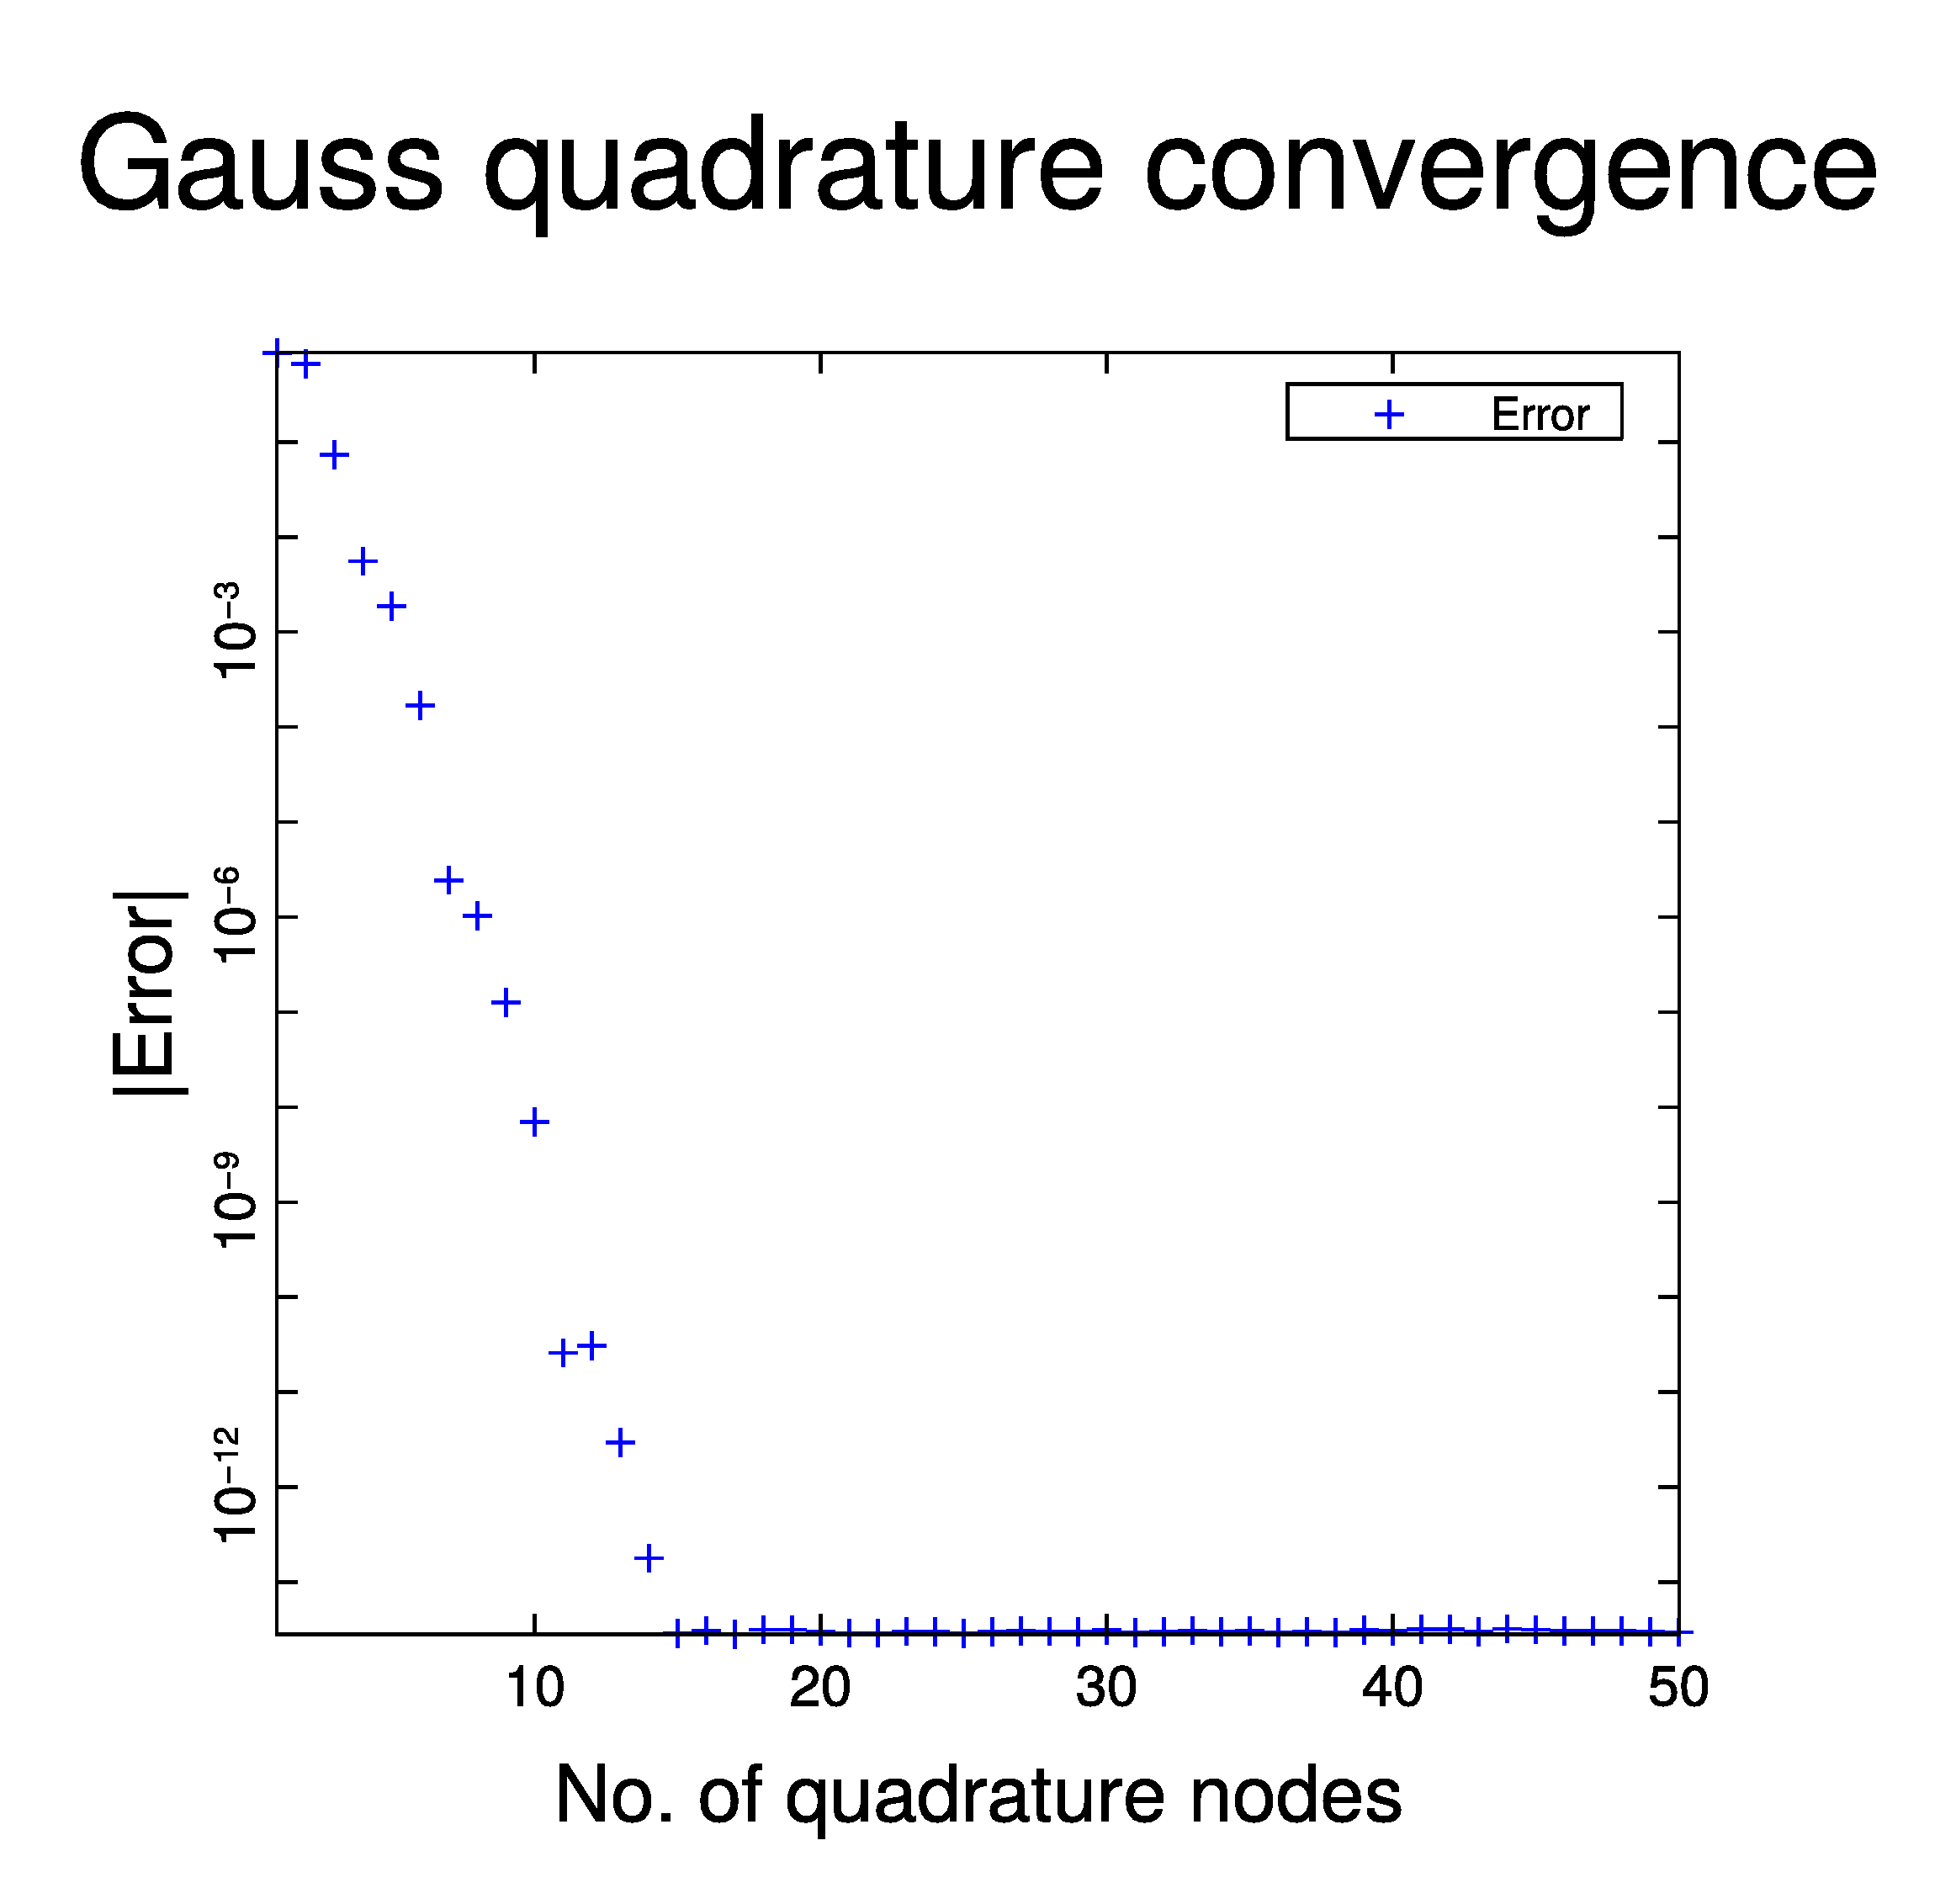
\includegraphics[width=0.6\textwidth]{\problems/ch_numericalquadrature/PICTURES/GaussConvCV.eps}
\caption{Convergence of \texttt{GaussConvCV.m}.}
\label{fig:GaussianQuadrature_GaussConvCV}
\end{figure}
\end{solution}
\end{subproblem}

%%%%%%%%%%%% SUBPROBLEM 5
\begin{subproblem}[3] \label{subprb:GaussianQuadrature_5}
Explain the difference between the results obtained in subtasks \ref{subprb:GaussianQuadrature_1} and \ref{subprb:GaussianQuadrature_4}.

\begin{solution}
The convergence is now exponential.
The integrand of the original integral belongs to $C^0([-1,1])$ but not to $C^1([-1,1])$ because the derivative of the $\arcsin$ function blows up in $\pm1$.
The change of variable provides an analytic integrand: $x\cos(x)\sinh(\sin x)$.
Gauss quadrature ensures exponential convergence only if the integrand is analytic.
This explains the algebraic and the exponential convergence.
\end{solution}
\end{subproblem}

\end{problem}
